\documentclass{reportx}

\newcounter{csubsection}
\NewDocumentCommand\optmodule{sO{}mmm}{%
    \IfBooleanTF{#1}{%
        \begin{equation*}
            \ifthenelse{\equal{#2}{}}{}{(#2)\quad}
            \begin{aligned}
                \begin{cases}
                    #3 \quad & #4 \\
                    \mathrm{s.t.} \quad #5
                \end{cases}
            \end{aligned}
        \end{equation*}
    }{%
        \begin{equation}
            \ifthenelse{\equal{#2}{}}{}{(#2)\quad}
            \begin{aligned}
                \begin{cases}
                    #3 \quad & #4 \\
                    \mathrm{s.t.} \quad #5
                \end{cases}
            \end{aligned}
        \end{equation}
    }%
}

\begin{document}
    % \nocite{*}

    \section{文献情况介绍及实验内容}

工业控制系统(Industrial Control Systems,ICS)广泛应用于电力、制造、水利等关键基础设施,其安全性和稳定性至关重要。
一旦ICS受到攻击,可能会造成严重的损坏。
因此,ICS的异常检测是保障关键基础设施安全的核心任务。
传统异常检测方法主要关注单一域中的指标,如网络域中的网络流量或物理域中的传感器数据,但ICS中不同域(如传感器的物理状态、网络通信流量等)的行为存在强相关性,仅分析单一域难以全面识别异常。
随着ICS与互联网的深度融合,攻击者可通过多域协同攻击绕过传统单域检测机制。
例如,网络攻击可能导致传感器数据异常,但某些攻击仅影响物理设备而不改变网络流量。

现有的方法如基于RNN\cite{mandic2001recurrent}、GAN\cite{creswell2018generative}或基于单域图的神经网络模型无法有效建模跨域关联,导致检测精度不足和误报率高。
文章\cite{zhan2024anomaly}在GDN\cite{deng2021graph}的基础上提出了一种基于跨域表示学习的ICS异常检测方法(MGDN),该方法能够学习多域行为的联合特征,结合动态图结构学习与跨域交叉注意力机制,进一步提升多域异常检测的鲁棒性与实时性。

本文将进行如下工作:

第一,全面介绍MGDN模型的核心思想与整体架构。
具体包括多图构建方法、多图信息的融合策略、基于注意力机制的图卷积神经网络建模方式,以及最终融合输出的机制。
该部分将详细阐述如何通过构建多个表示不同语义关系的图,从而提升异常检测的表示能力和模型的泛化性能。

第二,深入探讨MGDN模型的优化策略。
本文将介绍多任务学习中的多梯度下降算法,给出其数学形式化定义,解释其在多任务场景下如何实现梯度的平衡与协调。
同时,本文将简要回顾多任务学习的发展历程。

第三,在SWaT数据集上开展模型性能评估实验。
通过与九种代表性的基线模型进行系统对比,从准确率、召回率、F1分数等多个维度评估MGDN的优势。此外,还将通过不同优化器的对比实验,进一步验证多梯度下降算法在MGDN中的关键作用和性能提升效果。

    \section{算法实现及改进}

文章提出一种跨域图表示学习方法。核心思想是通过构建多域图结构,将不同域的行为特征统一编码。
该方法结合不同域的数据,利用注意力机制图卷积网络(Graph Convolutional Networks,GCN)\cite{kipf2017semi}学习共享与域特定特征。
模型框架如\cref{figure:跨域表示学习的总体框架}所示。

\begin{figure}[ht]
    \centering
    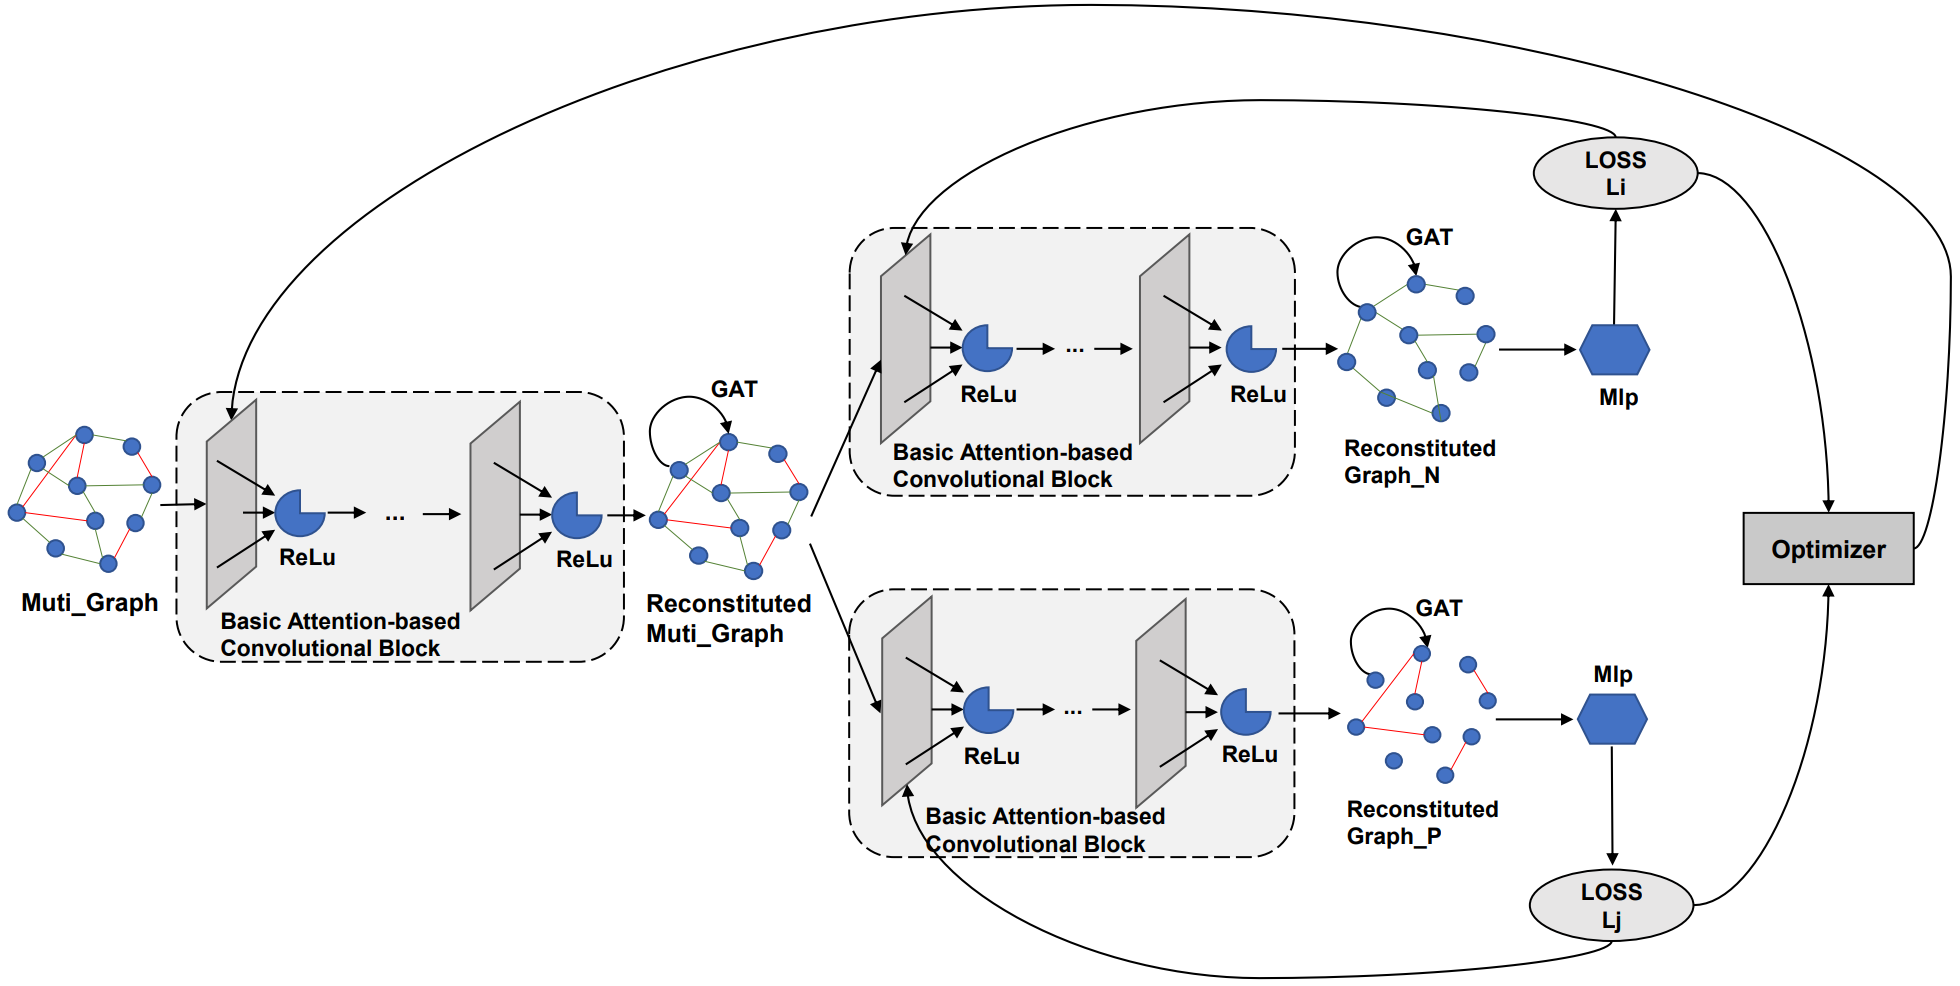
\includegraphics[width=1\textwidth]{img/跨域表示学习的总体框架.png}
    \caption{跨域表示学习的总体框架}
    \label{figure:跨域表示学习的总体框架}
\end{figure}

\subsection{多图构建}

在该方法中,目标是从ICS的多个域(如物理域、网络域等)中提取节点特征,并构建统一的多图结构用于跨域建模。
多图表示结构的构构建过程如\cref{figure:多图表示结构的构建过程}所示。

\begin{figure}[ht]
    \centering
    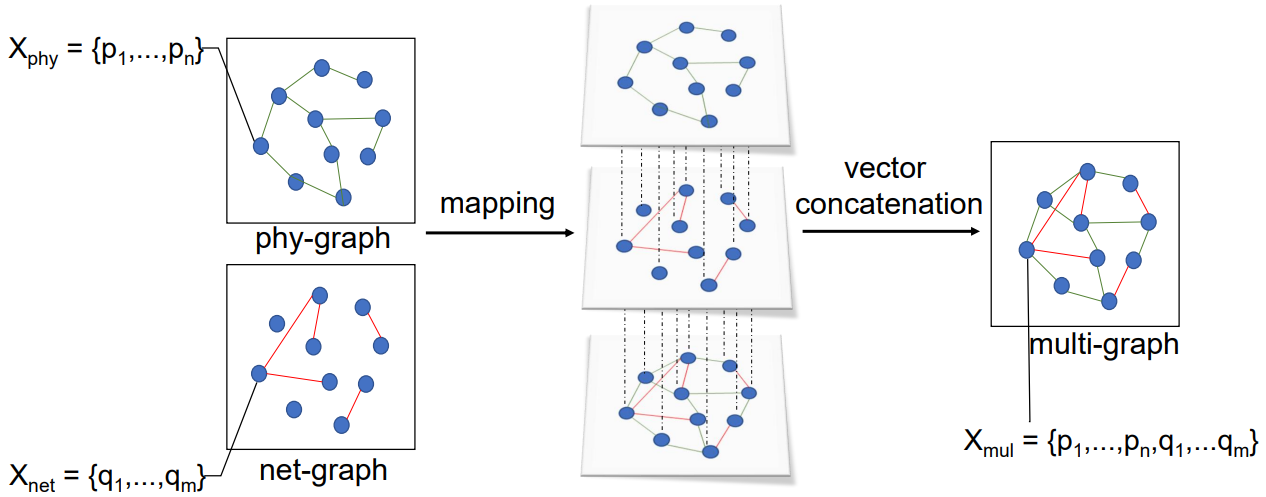
\includegraphics[width=1\textwidth]{img/多图表示结构的构建过程.png}
    \caption{多图表示结构的构建过程}
    \label{figure:多图表示结构的构建过程}
\end{figure}

假设有$n$个节点(传感器和执行器),来自不同域的数据被统一为相同的时间粒度(如秒级粒度),每个节点在第$d$个域上的特征矩阵为
\begin{equation*}
    \bm{x}^{(d)}\in\mathbb{R}^{n\times t} \text{,}
\end{equation*}
其中$t$为时间步长。

对每个域$d\in\{1,2,\cdots,D\}$, 构建一个无向加权图
\begin{equation*}
    \mathcal{G}_d=\left<\mathcal{V},\mathcal{E}_d\right> \text{,}
\end{equation*}
其中$\mathcal{V}$表示所有节点的集合,且$|\mathcal{V}|=n$,$\mathcal{E}_d$为第$d$个域中的边集合。

节点之间的边权通过余弦相似度计算其嵌入向量之间的相似性。
对于任意两个节点$i$和节点$j$,在第$d$域的嵌入向量为$\bm{v}_i^{(d)}$和$\bm{v}_j^{(d)}$,则计算节点$i$到节点$j$的边权
\begin{equation*}
    e_{ij}^{(d)}=\frac{\left(\bm{v}_i^{(d)}\right)^\mathrm{T}\bm{v}_j^{(d)}}{\left\|\bm{v}_i^{(d)}\right\|\left\|\bm{v}_j^{(d)}\right\|} \text{,}
\end{equation*}
之后使用Top-k策略筛选每个节点最相关的$k$个邻居构建图$\mathcal{G}_d$,进一步融合成多图结构
\begin{equation*}
    \mathcal{G}=\left<\mathcal{V}, \textstyle\bigcup_{i=1}^d\mathcal{E}_i\right> \text{,}
\end{equation*}
节点$i$的跨域特征向量表示为
\begin{equation*}
    \bm{v}_i=\bm{v}_i^{(1)}\oplus\bm{v}_i^{(2)}\oplus\cdots\oplus\bm{v}_i^{(D)} \text{。}
\end{equation*}

\subsection{基于注意力机制的图卷积神经网络建模}

文章引入GDN中的图注意力机制(Graph Attention Network, GAT)\cite{velickovic2018graph}对节点信息进行聚合,捕捉局部邻居中的非均匀关系。

首先,定义节点$j$对节点$i$的注意力权重
\begin{equation*}
    \alpha_{ij}=\mathrm{Softmax}\left(\mathrm{LeakeyReLU}\left(\bm{a}^\mathrm{T}(\bm{v}_i\oplus\bm{v}_j)\right)\right) \text{,}
\end{equation*}
其中$\bm{a}$为可学习的向量。则节点$i$的聚合表示更新为
\begin{equation*}
    \bm{z}_i=\mathrm{ReLU}\left(\alpha_{ii}\bm{W}\bm{v}_i+\bm{W}\sum_{j\in\mathcal{N}_i}\alpha_{ij}\bm{v}_j\right) \text{,}
\end{equation*}
其中$\bm{W}$为可学习的矩阵。

\subsection{融合输出}

使用节点的聚合表示和特征向量进行输出,即
\begin{equation*}
    \hat{\bm{y}}=f_\theta([\bm{z}_1\circ\bm{v}_1, \bm{z}_2\circ\bm{v}_2, \cdots, \bm{z}_n\circ\bm{v}_n]) \text{,}
\end{equation*}
其中$\circ$为逐元素乘法,$f_\theta$为多层感知机。

    \section{核心优化思想及其发展历程}

\subsection{优化思想}

为了在多个域(如物理域、网络域等)上同时优化预测性能,文章使用了多任务学习(Multi-Task Learning, MTL)\cite{ruder2017overviewmultitasklearningdeep}方法,其目标是联合优化每个任务的损失
\begin{equation*}
    \min_{\bm{W}_s,\bm{W}_1,\bm{W}_2,\cdots,\bm{W}_D}\sum_{d=1}^D\beta_d\mathcal{L}_d(\bm{W}_s,\bm{W}_d) \text{,}
\end{equation*}
其中$\bm{W}_s$为共享层参数,$\bm{W}_d$、$\mathcal{L}_d$和$\beta_d$分别为第$d$域的专属参数、损失函数及任务权重。

为了解决梯度冲突问题,引入了多梯度下降算法(Multiple Gradient Descent Algorithm,MGDA)\cite{desideri2012multiple},其基本思想是寻找一组权重$\{\gamma_d\}$,使得多个损失函数在共享参数$\bm{W}_s$上的梯度方向可以共同优化,即
\optmodule{\min_{\gamma_1,\gamma_2,\cdots,\gamma_D}}{\left\|\sum_{d=1}^D\gamma_d\nabla_{\bm{W}_s}\mathcal{L}_d(\bm{W}_s,\bm{W}_d)\right\|^2}{
    &\sum_{d=1}^D\gamma_d=1\text{,} \\
    &\gamma_1,\gamma_2,\cdots,\gamma_D\geq0\text{,}
    \label{equation:MGDA}
}
该优化问题保证在共享参数更新中不会偏向某一特定任务。

当$D=2$时,\cref{equation:MGDA}简化为
\optmodule*{\min_{\gamma}}{\left\|\gamma\nabla_{\bm{W}_s}\mathcal{L}_1(\bm{W}_s,\bm{W}_1)+(1-\gamma)\nabla_{\bm{W}_s}\mathcal{L}_2(\bm{W}_s,\bm{W}_2)\right\|^2}{
    &\gamma\geq0\text{。}
}

\subsection{MTL的发展历程}

多任务学习的思想可以追溯到上世纪90年代,其中最具代表性的开创性工作来自于Rich Caruana在1997年的论文\cite{caruana1997multitask}。
这篇文章明确提出了一个基本设想:如果我们同时学习多个相互关联的任务,就可以通过共享表示来提升模型的泛化能力。
这一时期的多任务学习主要关注于参数共享的形式,也就是通过设计模型结构,让多个任务共享一部分网络参数(例如前几层),而在高层则保留各自的特定参数。
这样的设计既利用了任务间的相关性,又保留了个性化特征。

随着深度学习的发展,特别是CNN和RNN等结构的广泛应用,多任务学习进入了“深度MTL”时代。
研究者开始思考不仅仅是共享前几层的问题,而是如何更加灵活地在网络中进行共享。
例如,Cross-Stitch Networks\cite{misra2016cross}、Sluice Networks\cite{ruder2019latent}等进一步提出了“选择性共享”的策略,即网络的每一层都可以决定是否共享,这种方式使得模型在面对任务相关性强弱不一的场景时具有更大的灵活性。

但是,这一时期很快暴露出一个重要问题:共享结构设计虽然能够在一定程度上提高性能,但很多时候,多任务学习的训练过程并不稳定。
有时候,模型在优化某个任务时,会影响甚至破坏另一个任务的性能。这种现象在训练过程中表现为任务之间的“负迁移”或“梯度冲突”。
任务的损失函数虽然在理论上可以共同最小化,但在梯度空间中,它们的方向可能是彼此冲突的。
这就催生了人们对多任务优化策略本身的深入研究。

真正把这个问题提升到理论高度的是文章\cite{desideri2012multiple,sener2018multi}。
文章将多任务学习转化为一个经典的多目标优化问题(Multi-objective Optimization, MOO),即在参数空间中同时最小化多个目标函数,而不是对它们进行简单的加权求和。
他们引入了Pareto最优的概念,认为多任务学习的本质是找到一个所有任务都“无法进一步改善而不损害其他任务”的平衡点。

MGDA 的核心思想是,每次参数更新时都不直接沿着所有梯度简单平均的方向走,而是求解一个最小范数问题,在所有任务的梯度凸包中找到一个合适的组合方向,使得整体更新方向在几何意义上最“中性”、最“折中”。
这个方向被视为当前任务之间最合理的优化方向,从而避免了梯度冲突的直接影响。
该方法提出后,迅速成为多任务优化的核心代表方法之一。

到今天,多任务学习已经不再只是“如何共享参数”这样一个模型结构设计问题,更是一个“如何优化更新”的动态策略问题。
MGDA作为第一个明确从优化角度重新定义MTL训练流程的方法,为后续梯度调度类方法打开了方向,构建了以“Pareto最优”为核心思想的全新视角。

    \section{实验设置、数据集及结果分析}

文章使用SWaT(Secure Water Treatment)\cite{mathur2016swat}数据集进行实验。
该数据集由新加坡科技设计大学(Singapore University of Technology and Design,SUTD)网络安全研究中心的iTrust实验室发布,模拟了真实水处理系统的运行场景。
数据集包含51个物理传感器(如流量计、阀门状态)和16个网络特征(如数据包数量、协议类型),时间跨度为11天,前7天为正常操作,后4天注入41种攻击。
\cref{table:swat static info}总结了SWaT数据集在物理和网络领域的统计数据。

文章使用准确率(Precision)、召回率(Recall)、假阳性率(False Positive Rate,FPR)和F1分数评估模型性能,这些指标的计算公式如下:
\begin{align*}
    &\mathrm{Precision}=\frac{\mathrm{TP}}{\mathrm{TP}+\mathrm{FP}} \text{,} \\
    &\mathrm{Recall}=\frac{\mathrm{TP}}{\mathrm{TP}+\mathrm{FN}} \text{,} \\
    &\mathrm{FPR}=\frac{\mathrm{FP}}{\mathrm{FP}+\mathrm{TN}} \text{,} \\
    &\mathrm{F1}=\frac{2\times\mathrm{Precision}\times\mathrm{Recall}}{\mathrm{Precision}+\mathrm{Recall}} \text{。}
\end{align*}
实验结果如\cref{table:matrics of mgdn and the baseline methods}所示。

\begin{table}[ht]
    \centering
    \caption{SWaT数据集在不同域中的统计数据}
    \label{table:swat static info}
    \begin{tabular}{ccccc}
        \toprule
        \textbf{域} & \textbf{训练数据} & \textbf{训练数据条目} & \textbf{特征数} & \textbf{异常率} \\
        \midrule
        物理域 & 21,830 & 34,201 & 51 & 16.61\% \\
        网络域 & 21,830 & 34,201 & 3  & 16.61\% \\
        \bottomrule
    \end{tabular}
\end{table}

\begin{table}[ht]
    \centering
    \caption{MGDN与基线方法的评价指标}
    \label{table:matrics of mgdn and the baseline methods}
    \begin{tabular}{ccccc}
        \toprule
        \textbf{Method} & \textbf{FPR (\%)} & \textbf{Precision (\%)} & \textbf{Recall (\%)} & \textbf{F1 (\%)} \\
        \midrule
        DTAAD       & 13.33 & 59.88 & 99.99 & 74.90 \\
        GDN         & 10.70 & 64.91 & 99.45 & 78.55 \\
        LSTM-AD     & 13.33 & 59.88 & 99.99 & 74.90 \\
        MAD-GAN     & 13.57 & 59.45 & 99.99 & 74.57 \\
        MSCRED      & 13.33 & 59.89 & 99.99 & 74.91 \\
        MTAD-GAT    & 13.39 & 59.78 & 99.99 & 74.83 \\
        OmniAnomaly & 13.36 & 59.83 & 99.99 & 74.87 \\
        TranAD      & 13.35 & 59.85 & 99.99 & 74.88 \\
        USAD        & 13.26 & 60.02 & 99.99 & 75.01 \\
        \textbf{MGDN}   & \textbf{3.07} & \textbf{84.65} & \textbf{85.12} & \textbf{84.88} \\
        \bottomrule
    \end{tabular}
\end{table}

\begin{table}[!ht]
    \centering
    \caption{不同多目标优化器下的评价指标}
    \label{table:matrics of opt}
    \begin{tabular}{cccc}
        \toprule
        \textbf{Method} & \textbf{Precision (\%)} & \textbf{Recall (\%)} & \textbf{F1 (\%)} \\
        \midrule
        0.25, 0.75  & 49.30 & 84.46 & 62.28 \\
        0.5, 0.5    & 83.15 & 82.34 & 83.87 \\
        0.75, 0.25  & 80.99 & 83.39 & 82.79 \\
        \textbf{MGDA}        & \textbf{84.65} & \textbf{85.12} & \textbf{84.88} \\
        \bottomrule
    \end{tabular}
\end{table}

将多梯度优化器更换成基于静态权重的梯度优化器,并分别设置不同的权重。
从\cref{table:matrics of opt}中可以看出,将物理域和网络域的损失权重分别设定为0.5和0.5能够取得比其他静态权重方法更好的效果,但仍然比使用MGDA的模型的F1低1.01\%。
因此,引入多梯度下降优化算法有利于模型更好地动态调整。

    \section{结论}

文章提出了一种基于跨域表示学习的异常检测方法,该方法将多个域的ICS数据结合起来进行跨域学习和异常检测。
通过物理域与网络域数据的联合建模,克服了单领域分析的局限性。注意力机制与多任务优化的结合,使模型在保留领域特征的同时捕捉跨域关联。
文章在大规模的真实世界数据集上对模型进行了评估,实验结果表明文章的模型优于基准模型。
此外,文章的模型能够更好地平衡减少误报和提高异常检测精度之间的关系,提供了一个更实用和理想的ICS异常检测模型。


    \stepcounter{section}
    \renewcommand{\refname}{\chinese{section}、参考文献}

    \phantomsection
    \addcontentsline{toc}{section}{参考文献}
    \bibliography{references}
\end{document}
